\section{引言}

\subsection{研究背景及意义}
当一用户打开大众点评想要搜索家附近的咖啡厅时,用户不仅提供了查询内容,还包括其位置信息,这类查询称为空间关键字查询\cite{DBLP:conf/sigmod/ChenSM06,DBLP:journals/pvldb/CongJW09,DBLP:conf/icde/FelipeHR08, DBLP:conf/ssdbm/HariharanHLM07,DBLP:conf/dexa/KhodaeiSL10, DBLP:conf/cikm/ZhouXWGM05,DBLP:journals/tkde/LiLZLLW11,DBLP:conf/sigmod/LuLC11,DBLP:conf/ssd/RochaGJN11,DBLP:journals/vldb/WuCJ12,DBLP:journals/tkde/WuYCJ12,DBLP:journals/tods/WuYJ13}。空间关键字查询的信息是多维度的,不仅表示了用户搜索目标,还指定了空间信息,例如街道地址、邮政编码或纬度和经度等地理坐标。图\ref{top5object}展示了一个空间关键字查询示例。图中的黑点表示查询位置,查询内容为“便利店”。该查询基于一个评分函数,对充电桩的距离和文本相关性进行加权求和,返回排名前5位的便利商店,在图中用正方形表示。空间关键词查询广泛地应用在商业环境中中,例如,为了适应移动互联网下搜索对象的变化,Google推出了一系列变革的搜索项目,Google Now就是其中一个。Google Now会记录用户的动态行为以满足他们未来的搜索需求,比如,该软件会记录用户开车的行为以及是否停止驾驶或离开车子,避免用户忘记车子停那里。
\begin{figure}[htbp]
	% caption放上面就会显示在图的上方,出现在下面就是出现在图的下方
	% label的位置也有讲究
	\begin{center}
		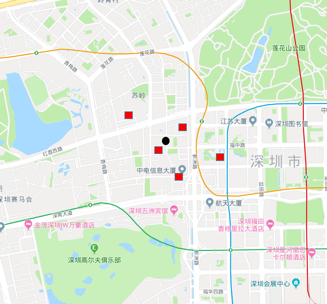
\includegraphics[width=3in]{top5object.png}
		\caption{Top-5对象}
		\label{top5object}
	\end{center}
\end{figure}

近年来,有几项基于空间关键字查询的研究,但它们在查询参数和评分函数上有所不同。连续移动空间的top-k关键字查询\cite{DBLP:journals/tods/WuYJ13,DBLP:conf/icde/WuYJC11}在查询位置不断变化下返回最新的结果;位置感知型的top-k权威文本检索查询\cite{DBLP:journals/pvldb/CaoCJ10}对权威对象的邻近对象给予高排名;集合空间关键字查询\cite{DBLP:conf/sigmod/CaoCJO11}检索一组与查询关键字匹配的对象;RochaJunior和Nørvåg\cite{DBLP:conf/edbt/Rocha-JuniorN12}考虑公路网络空间下的关键词搜索;李\cite{DBLP:conf/icde/LiFX12}研究移动方向下的空间关键字搜索。但是大多数现有的研究以单个对象作为结果对象。然而在空间关键字查询中,用户可能更感兴趣的是满足查询需求的区域,例如,对于一个想要找“川菜餐厅”的用户来说,一组距离远且分散的餐厅推荐显然不是他想获得的结果。事实上,这些在空间上彼此靠近,文本相似的对象之间往往能够构成小型区域,显示出区域性特征。而空间文本聚类便是在无监督条件下找出这些区域,称为“簇”。

聚类是数据挖掘领域中一种无监督地组织和管理信息的技术之一。空间文本聚类以文本信息为特征、空间关键词查询信息为约束条件,使用相似度计算将具有相似属性但无类别标记的文本信息聚类在一起。

因此如何利用空间关键字查询所体现的区域性,从海量的数据中有效提取信息并将其按特征划分是大数据时代下一个重要的研究问题。

\subsection{研究目的与主要工作}
以往的研究\cite{DBLP:journals/pvldb/ChoiCT12,DBLP:conf/cikm/LiuYS11,DBLP:journals/pvldb/TaoHCC13}考虑目标与检索区域的共定位关系,使结果区域内的目标总权重最大化的同时使结果区域限定为特定的形状(固定大小的矩形或圆形)。另外一项研究\cite{DBLP:conf/cikm/WuJ16}提出了一个支持探索性用户行为的解决方案,并且聚类结果没有形状约束。该研究提出一种新型的查询,即top-k空间文本簇(k-STC)查询,该查询结果将返回top-k簇, 满足(i)每个簇包含与查询关键词语义相关的对象,(ii)每个簇的密度满足用户给出的约束,以及(iii)根据到用户地理位置的距离以及与查询关键字的语义相关性对符合查询要求的簇排序。图\ref{top5cluster}是k-STC查询的示例,查询位置和关键字与图\ref{top5object}一致,结果簇展示在图中。
\begin{figure}[htbp]
	% caption放上面就会显示在图的上方,出现在下面就是出现在图的下方
	% label的位置也有讲究
	\begin{center}
		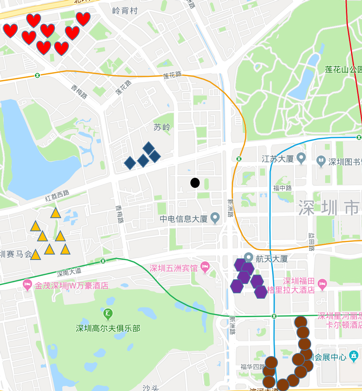
\includegraphics[width=3in]{top5cluster.png}
		\caption{Top-5簇}
		\label{top5cluster}
	\end{center}
\end{figure}

k-STC引入IR-树存储空间对象及其文本描述,依据关键词从IR-树上获取相关对象,通过聚类算法将相关对象形成簇。簇的形成依赖于参数,簇的排名依赖于评分函数。k-STC采用基于密度的聚类算法,找到由核心对象及其密集邻域组成的簇。

本论文是对k-STC空间文本簇查询的进一步研究,设计并实现基于密度空间文本簇检索系统。主流的聚类算法有层次聚类、扁平聚类、基于密度的聚类、基于网格的聚类等,本论文采用基于密度的聚类算法,优点是(1)聚类结果不受距离限制;(2)不需要指明聚类数量;(3)对异常值具有健壮性。另外,本论文还将针对空间对象数量大,遍历IR-tree检索对象耗时的问题,引入带有词项权重的索引文件,使检索系统能够更快的找到优异的簇,提高检索效率。并通过实验验证系统的性能和优化效果。

主要的工作流程如下:
\begin{itemize}
	\item 收集空间文本数据
	\item 设计并实现基于密度的空间文本检索系统
	\item 根据优化方案,对系统进行优化
	\item 测试系统并评估实验结果
\end{itemize}

\subsection{国内外相关研究}
本论文主要涉及到两个技术:空间文本搜索(1.3.1)和聚类算法(1.3.2)。本小节将分别介绍这两个技术在国内外的相关研究。


\subsubsection{空间文本搜索}
空间关键词查询近年来引起了广泛的关注。目前已经提出了几种有效的地理文本索引来支持空间关键字查询。大多数索引结合了用于空间索引的R树和用于文本查询的倒排索引表,例如IR2$^2$-树\cite{DBLP:conf/icde/FelipeHR08}、IR-树\cite{DBLP:journals/vldb/WuCJ12}和S2I\cite{DBLP:conf/ssd/RochaGJN11}。这些混合索引结构能够在处理查询时利用空间信息和文本信息来修剪搜索空间。

不同的空间关键字查询研究会采取不同的得分函数,这些得分函数决定了查询参数和如何确定对象与查询参数的相关性。例如,连续移动top-k 空间关键字查询\cite{DBLP:journals/tods/WuYJ13, DBLP:conf/icde/WuYJC11};基于权重的位置感知top-k文本检索查询\cite{DBLP:journals/pvldb/CaoCJ10};集合空间关键字查询\cite{DBLP:conf/sigmod/CaoCJO11};RochaJunior和Nørvåg\cite{DBLP:conf/edbt/Rocha-JuniorN12}考虑了道路网络中的空间关键词搜索;Li等人\cite{DBLP:conf/icde/LiFX12}研究了受运动方向约束的空间关键词搜索等。

还有一系列研究了满足不同用户需求的空间关键字查询研究。Chen等\cite{DBLP:conf/sigmod/ChenCC13}研究了如何将连续输入的布尔范围查询流与实时传入的地理文本对象流进行匹配的问题。关键字感知最优路由查询\cite{DBLP:journals/pvldb/CaoCCX12}找到了一个包含用户指定的一组关键字,满足指定的预算约束,并根据特定的评分函数获得最佳的评分的最优路由。集合空间关键字查询\cite{DBLP:journals/tods/CaoCGJO15,DBLP:conf/sigmod/CaoCJO11,DBLP:conf/sigmod/LongWWF13}查找一组对象,这些对象靠近一个查询点,并且集合包含一组查询关键字。Wu等\cite{DBLP:journals/tods/WuYJ13, DBLP:conf/icde/WuYJC11}研究了用户(查询位置)连续移动时,top-k空间关键字查询结果集的维护问题。反向空间文本k最近邻(RSTkNN)查询\cite{DBLP:conf/sigmod/LuLC11}找到的对象是将查询对象作为它们k个空间文本最相似的对象之一

最近的研究\cite{DBLP:journals/pvldb/BoghSJ13,DBLP:journals/vldb/SkovsgaardJ15}针对的是用户希望找到与查询关键字相关的附近兴趣点集合的情况,部分用户希望在做出某些决定(诸如购买特定产品之类)之前,可以方便地探索若干个选项,而上述的集合便可以满足这类用户的需求。Zhang等\cite{DBLP:conf/icde/ZhangOT10, DBLP:conf/icde/ZhangCMTK09}研究的查询采用一组关键字,目标是找到一组地理文本对象,使其文本描述的联合覆盖所有的查询关键字,并使对象的直径最小化。考虑到对象之间的共定位关系,应当检索区域使得结果区域内的对象的总权重最大化\cite{DBLP:journals/pvldb/ChoiCT12,DBLP:conf/cikm/LiuYS11,DBLP:journals/pvldb/TaoHCC13}。最近的一项研究\cite{DBLP:journals/pvldb/CaoCJY14}计算了一个最大和区域,该区域的对象之间的公路网距离小于查询约束,得分之和最大。但是这种查询会检索到一个包含许多低分对象的区域,而忽略一个包含少数高分对象的区域。此外,该研究的查询为范围查询,减小了搜索空间,因而如果当查询范围覆盖整个数据集时,性能是不确定的。

\subsubsection{聚类算法}
聚类算法体系一般划分为扁平聚类、层次聚类、基于密度的聚类,基于网格的聚类等等\cite{DBLP:journals/coling/Vechtomova09}。聚类算法的选择决定了聚类结果的状态和效率。

扁平聚类通过迭代重定位将文本集中的n个文本分配到K个簇中,使得同一个簇的对象满足“相关”关系,不同簇的对象满足“相异关系。最典型的算法有K-均值算法。针对聚类结果对中心敏感,k值无法确定这一问题,汤叶青\cite{DBLP:tyq}提出了一种改进的K-means算法和K值学习算法。K值学习算法引入遗传算法,根据适应度函数,不断通过遗传操作进行迭代找到最佳聚类数。

层次聚类依据自顶向下或自底向上可以分为凝聚式或分裂式。凝聚式的基本思路是:先将每个文档看做一个簇, 然后不断对簇进行两两合并,直到所有的文档聚成一类。分裂式的基本思路是:先将所有文档看做一个簇,然后不断对簇进行分裂知道每篇文档都成为一个簇。扁平聚类和层次聚类依据对象间的聚类进行聚类,因而聚类只能为固定的球形。

在基于密度的聚类中,簇是具有较高对象密度的区域。在稀疏区域内的对象通常被认定为噪点或边界对象。最常用的基于密度的聚类方法是DBSCAN\cite{DBLP:conf/kdd/EsterKSX96},该方法基于一定距离内的物体相互连接的阈值的定义了一个簇模型,称为“密度-可达性”。簇由所有密集连接的对象以及所有位于这些对象阈值距离内的对象组成,并且簇可以具有任意形状。OPTICS\cite{DBLP:conf/sigmod/AnkerstBKS99}是DBSCAN的一种推广,它不需要选择适当的范围参数,生成与连锁聚类相关的分层结果。DBRS\cite{DBLP:conf/pakdd/WangH03}通过反复随机选取一个非分类点并检查其邻域来改进DBSCAN。VDBSCAN\cite{DBLP:conf/icde/ZhangOT10}针对变密度数据集进行分析。在采用传统的DBSCAN算法之前,一些方法是根据k-dist图选择不同密度的几个参数ε值。在ε值不同的情况下,可以同时找到密度不同的簇。GDBSCAN根据点对象及其空间属性和非空间属性对点对象和空间扩展对象进行聚类。而基于密度的聚类能够发现任意形状的簇。基于密度的聚类判断一个簇的区域内是否达到阙值,小于阙值将被忽略,而大于阙值可以继续扩展。这样便有效地过滤了噪点。
